\documentclass{beamer}
% Language/Font package
\usepackage[utf8]{inputenc}
\usepackage[francais]{babel}
\usepackage[T1]{fontenc}

% Base package
\usepackage{graphicx}
\usepackage{color}
\usepackage{listings}
\usepackage{hyperref}

\usepackage{comment}

% Configuration
\definecolor{ligthYellow}{RGB}{255,255,229}

\lstset{
language=bash,
%numbers=left,
%numberstyle=\small,
%numbersep=8pt,
basicstyle=\small\ttfamily,
tabsize=2,
showspaces=false,
showstringspaces=false,
stringstyle=\color{red}\ttfamily,
commentstyle=\color{green}\ttfamily,
breaklines=true,
frame = single,
%framexleftmargin=15pt,
backgroundcolor=\color{ligthYellow}}

% Theme https://github.com/matze/mtheme
\usetheme[progressbar=frametitle]{metropolis}

% Title
\title{Présentation Git}
\subtitle{Un outil de collaboration puissant}
\date{\today}
\author{Denis Pettens \and Pablo Gonzalez Alvarez \and Gaëtan Cassiers}
\institute{Louvain-li-Nux}
\titlegraphic{\hfill
\includegraphics[height=2cm]{img/logo.png}}

\begin{document}

% slides pré-atelier pour les personnes en avance
\begin{frame}
\begin{center}
  Suivez cette présentation sur votre ordinateur :
   \vspace{1cm}
  \fbox{\Large\url{http://bit.ly/2mlKcv8}}
\end{center}

Préparez-vous à utiliser \texttt{git} :
\begin{itemize}
    \item Sur les ordinateur Windows UCL ouvrez \texttt{git bash}
    \item Ou installez \texttt{git} sur votre ordinateur :
    \begin{itemize}
        \item \textbf{Ubuntu} : \lstinline{sudo apt-get install git}
        \item \textbf{OS X} : \url{https://sourceforge.net/projects/git-osx-installer/}
        \item \textbf{Windows} : \url{https://git-for-windows.github.io/}
    \end{itemize}
\end{itemize}
\end{frame}

\maketitle

\begin{frame}{Cette présentation}
    \begin{itemize}
        \item Cette présentation est sous license libre CC-BY 4.0.
        \item Vous pouvez télécharger les slides à l'addresse
            \url{https://github.com/louvainlinux/atelier-git}
        \item Les instructions pour les exercices sont à
        \url{https://github.com/louvainlinux/atelier-git/blob/master/instructions.md}.
    \end{itemize}
\end{frame}

\begin{frame}{Table des matières}

\setbeamertemplate{section in toc}[sections numbered]
\tableofcontents[hideallsubsections]

\end{frame}

\section{Introduction}

\begin{frame}{Gérer un projet}
Comment gérez-vous actuellement un projet ?

\begin{itemize}
    \item L'envoyer à travers un message sur Facebook, ... (\textbf{Très mauvaise idée})
    \item L'envoyer par mail (\textbf{Un peu moins})
    \item Utiliser une Dropbox, Google Drive, ... (\textbf{Déjà mieux mais toujours risqué ou manque de fonctionalités})
\end{itemize}

Solution : Utiliser un \textbf{système de gestion de version décentralisé}
(Distributed Version Control System (DVCS) pour les anglophiles).
\end{frame}

\begin{frame}{Un DVCS ?}
    \begin{itemize}
        \item \textbf{Version} Enregistre des \og{}instantanés\fg{} du projet.
        \item \textbf{Gestion} Revenir en arrière, voir des différences,
            fusionner des modifications.
        \item \textbf{Décentralisé} Chacun travaille sur sa copie, et on fusionne les modifications.
        \item \textbf{Projet} n'importe quel répertoire (\og dossier\fg). Donc n'importe quoi !
    \end{itemize}
\end{frame}

\begin{frame}{Et Git dans tout ça ?}
\begin{itemize}
    \item \texttt{Git} a été créé en 2005 par \textbf{Linus Torvalds} (auteur de \texttt{Linux});
\end{itemize}
Ses avantages:
\begin{itemize}
    \item Le plus connu et utilisé (90~\% du marché, communauté très présente);
    \item Vitesse;
    \item Facile d'utilisation mais aussi très puissant;
    \item Distribué (pas besoin de connexion internet tout le temps);
\end{itemize}

Ses inconvénients:
\begin{itemize}
    \item De nouveaux concepts
    \item Interface principale en ligne de commande
    \item Mais il existe aussi des interfaces graphiques
\end{itemize}
\end{frame}

\section{Instalation et configuration}
\begin{frame}{Installer Git}
\textbf{Ubuntu} : \lstinline{sudo apt-get install git}

\textbf{OS X} : \url{https://sourceforge.net/projects/git-osx-installer/}

\textbf{Windows} : \url{https://git-for-windows.github.io/}
\end{frame}

\begin{frame}[fragile]
\frametitle{Configuration de base}

Git a besoin de deux informations de base sur vous pour pouvoir travailler efficacement :

\begin{itemize}
\item \textbf{Nom et Prénom}
\begin{lstlisting}
git config --global user.name "Jules Dupont"
\end{lstlisting}

\item \textbf{Email}
\begin{lstlisting}
git config --global user.email "jules.dupont@email.fr"
\end{lstlisting}
\end{itemize}

L'option \lstinline{--global} permet de configurer \texttt{git} pour tous vos autres projets sur votre PC.
\end{frame}

\begin{frame}[fragile]
\frametitle{Configuration de base -- Éditeur de textes}
\textbf{Linux}\begin{lstlisting}
git config --global core.editor "gedit"
\end{lstlisting}\textbf{Windows}\begin{lstlisting}
git config --global core.editor "notepad"
\end{lstlisting}
\textbf{Mac}\begin{lstlisting}
git config --global core.editor "TextEdit"
\end{lstlisting}
\end{frame}

\section{Premier pas avec la ligne de commande}

\begin{frame}[fragile]
\frametitle{Ligne de commande (aka shell), késako?}
Où suis-je :
\begin{lstlisting}
$ pwd
\end{lstlisting}
Contenu du dossier actuel :
\begin{lstlisting}
$ ls
\end{lstlisting}
Se déplacer :
\begin{lstlisting}
$ cd <path> # aller a path
$ cd .. # remonter d'un dossier
\end{lstlisting}
\end{frame}

\section{Premier pas avec Git}

\begin{frame}
\frametitle{Concept: le \textbf{commit}}

\begin{center}
    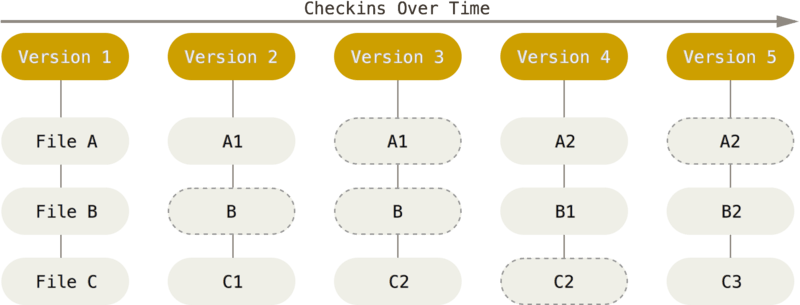
\includegraphics[width=0.9\textwidth]{img/commits.png}
\end{center}
\footnotesize{Les illustrations non-sourcées viennent de \url{https://git-scm.com/book}.}
\end{frame}

\begin{frame}[fragile]
\frametitle{Commande: git init}
\begin{itemize}
\item Initialise un dossier en un nouveau dépôt \texttt{git}.
\item Exemple
\begin{lstlisting}
$ mkdir newProject
$ cd newProject
$ git init
\end{lstlisting}
\item Cela crée un sous-dossier \texttt{.git} où tout la magie de git se fait
\item Vous mettrez tous les fichiers du projet dans \texttt{newProject}
\end{itemize}
\end{frame}

\begin{frame}[fragile]
\frametitle{Commande: git status}
\begin{itemize}
    \item \texttt{git} vous dit o\`u vous en êtes.
    \item Exemple
\begin{lstlisting}
$ git status
On branch master
Initial commit
nothing to commit (create/copy files and use "git add" to track)
\end{lstlisting}
\item À utiliser sans modération !
\end{itemize}
\end{frame}

\begin{frame}[fragile]
\frametitle{Commande: git add}
\begin{itemize}
    \item Ajoute un fichier dans le projet \texttt{git}.
    \item Exemple
\begin{lstlisting}
$ vi notes.txt # copier un fichier
$ git status
#[...]
Untracked files:
  (use "git add <file>..." to include in what will be committed)
  notes.txt
nothing added to commit but untracked files present (use "git add" to track)
$ git add notes.txt
#[...]
Changes to be committed:
  (use "git rm --cached <file>.." to unstage)
  new file:   notes.txt
\end{lstlisting}
\end{itemize}
\end{frame}

\begin{frame}[fragile]
\frametitle{Commande: git commit}
\begin{itemize}
    \item Crée un \texttt{commit} sur base des fichiers ajoutés.
    \item Exemple
\begin{lstlisting}
# toujours verifier ce qu'on commit
$ git status
#[...]
Changes to be committed:
  (use "git rm --cached <file>.." to unstage)
  new file:   notes.txt
$ git commit
# Ouvre un editeur de texte
# Editer, sauvegarder et fermer
[master (root-commit) 12f87b9] ajout de le premiere note
 1 file changed, 1 insertion(+)
\end{lstlisting}
\item Message de \texttt{commit}: décrit les changements effectués.
\end{itemize}
\end{frame}

\begin{frame}{En résumé: le cycle de vie d'un fichier}
\begin{figure}
    \centering
    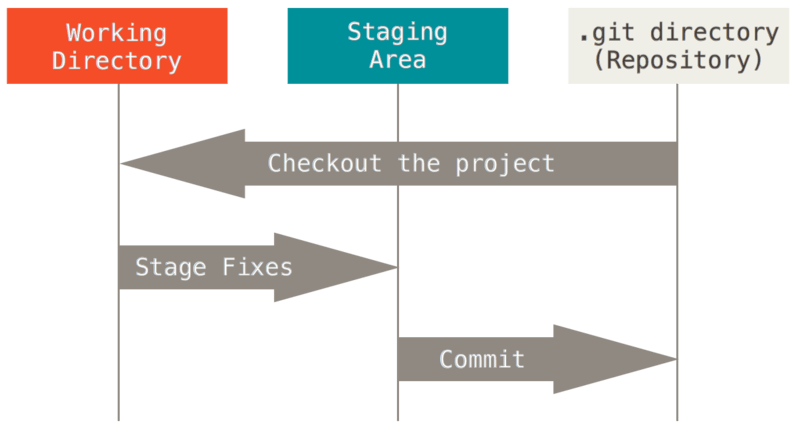
\includegraphics[width=\textwidth]{img/areas.png}
\end{figure}
\end{frame}

\begin{frame}[fragile]
\frametitle{Commande: git log}

\begin{itemize}
    \item Visualiser l'historique du projet
    \item Exemple
\begin{lstlisting}
$ git log
commit 12f87b95caff8cbeb5ce0717528d77e27
Author: Louvain Linux<info@louvainlinux.org>
Date:   Sun Feb 26 17:51:16 2017 +0100

    ajout de le premiere note
\end{lstlisting}
    \item Ouvre parfois un \texttt{pager}. Se déplacer avec les flèches haut/bas, quitter avec \texttt{q}.
\end{itemize}
\end{frame}

\begin{frame}[fragile]
    \frametitle{Astuce: de l'aide !}
    On peut trouver de l'aide:
    \begin{itemize}
        \item rapide: \texttt{git [command] -h}
\begin{lstlisting}
$ git log -h
usage: git log [<options>] [<revision-range>] [[--] <path>...]
   or: git show [<options>] <object>...

    -q, --quiet           suppress diff output
    --source              show source
[...]
\end{lstlisting}
        \item plus détaillée: \lstinline{git [command] --help}
    \end{itemize}
\end{frame}

\begin{frame}[fragile]
\frametitle{Exercice 1}
\begin{lstlisting}
$ mkdir newProject
$ cd newProject
$ git status
$ # Creer un fichier
$ git add monfichier.txt monfichier2.png
$ git commit
$ # Editer le message de commit
$ git log
\end{lstlisting}
Utile:
\begin{lstlisting}
$ git --help # liste des commandes git
$ git [commande] --help
\end{lstlisting}
Bonus: regardez l'aide de \texttt{git mv} et de \texttt{git rm}.
\end{frame}

\section{Les branches}

\begin{frame}{De derrière: les objets git}
    \begin{itemize}
        \item Chaque commit a un identifiant: \textbf{12f87}b95caff8cbeb5ce0717528d77e27db5669c.
    \end{itemize}
    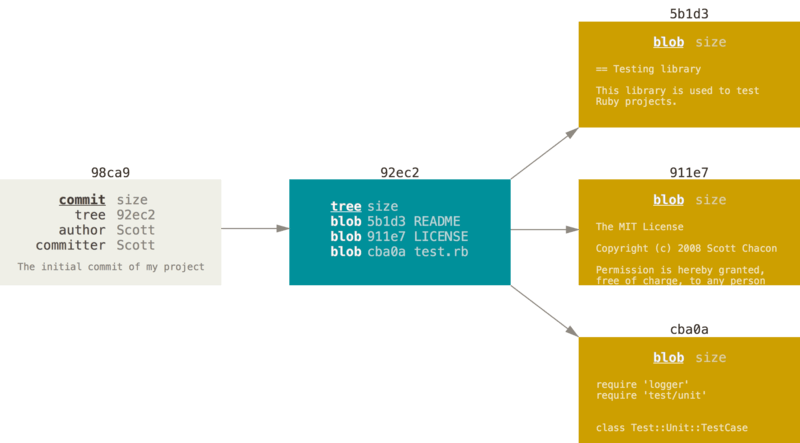
\includegraphics[width=0.8\textwidth]{img/commit-and-tree.png}
\end{frame}

\begin{frame}{De derrière: les parents}
    \begin{itemize}
        \item Chaque commit a un parent.
    \end{itemize}
    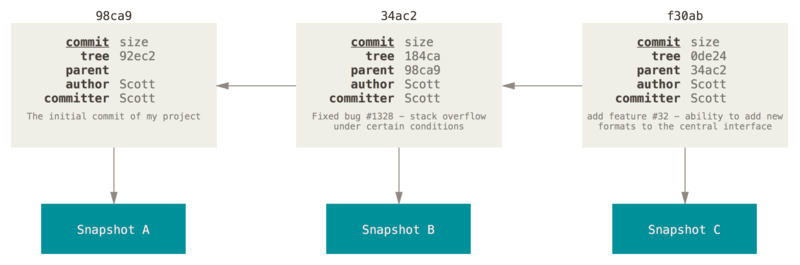
\includegraphics[width=\textwidth]{img/commits-and-parents.png}
\end{frame}

\begin{frame}{De derrière: les étiquettes}
    \begin{itemize}
        \item On peut mettre des étiquettes sur des commits.
        \item \texttt{HEAD} est la position actuelle.
    \end{itemize}
    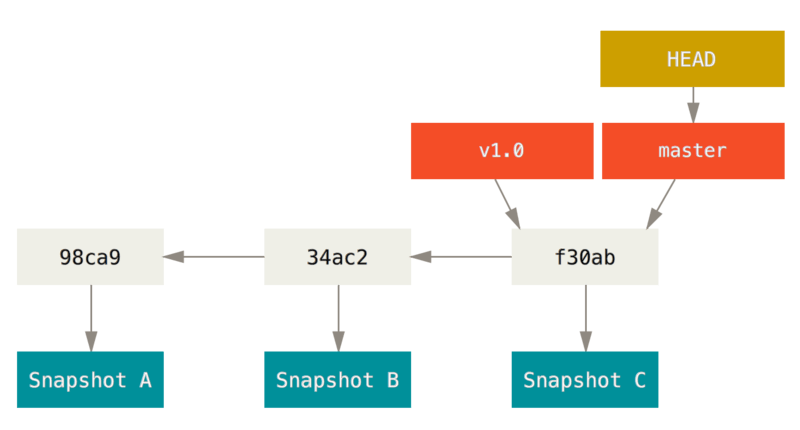
\includegraphics[width=\textwidth]{img/branch-and-history.png}
\end{frame}

\begin{frame}[fragile]
    \frametitle{Commande: git branch}
    \begin{itemize}
        \item Une branche est une nouvelle étiquette.
\begin{lstlisting}
$ git branch testing
\end{lstlisting}
        \item La branche par défaut est \texttt{master}.
    \end{itemize}
    \begin{center}
        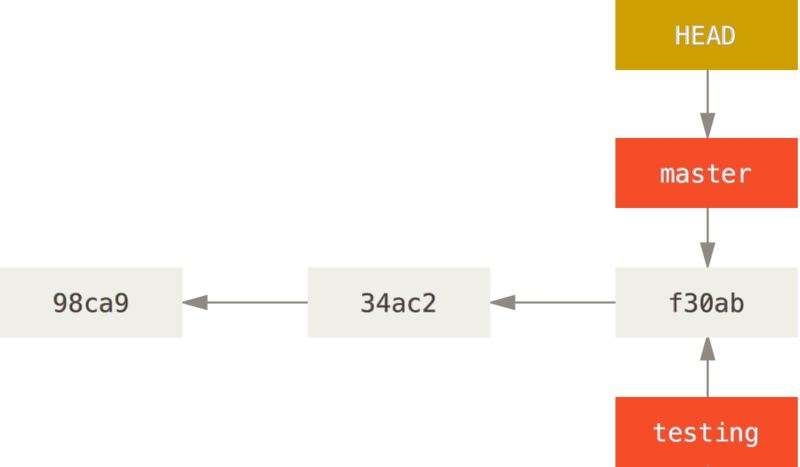
\includegraphics[width=0.8\textwidth]{img/head-to-master.png}
    \end{center}
\end{frame}

\begin{frame}[fragile]
    \frametitle{Commande: git checkout}
    \begin{itemize}
        \item Permet de changer de branche.
\begin{lstlisting}
$ git checkout testing
\end{lstlisting}
        \item La branche courante est celle qui suit les nouveaux commits.
    \end{itemize}
    \begin{center}
        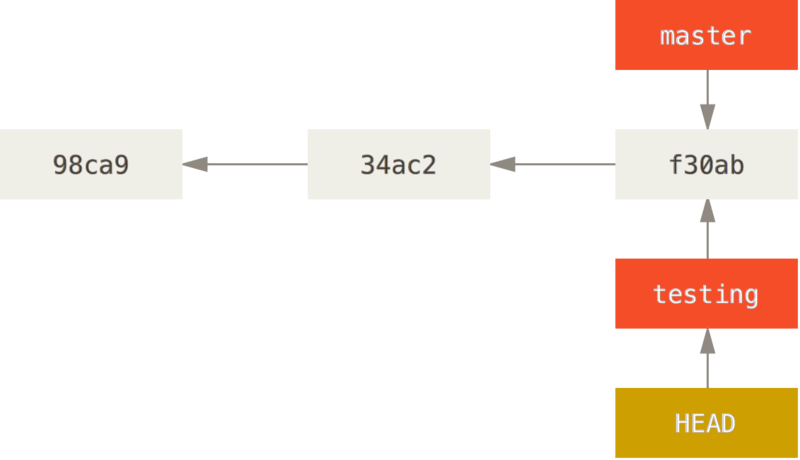
\includegraphics[width=0.8\textwidth]{img/head-to-testing.png}
    \end{center}
\end{frame}

\begin{frame}[fragile]
    \frametitle{Commande: git checkout (2)}
    \begin{itemize}
        \item La branche courante est celle qui suit les nouveaux commits.
    \end{itemize}
\begin{lstlisting}
$ [Quelques changements]
$ git commit
\end{lstlisting}

    \begin{center}
        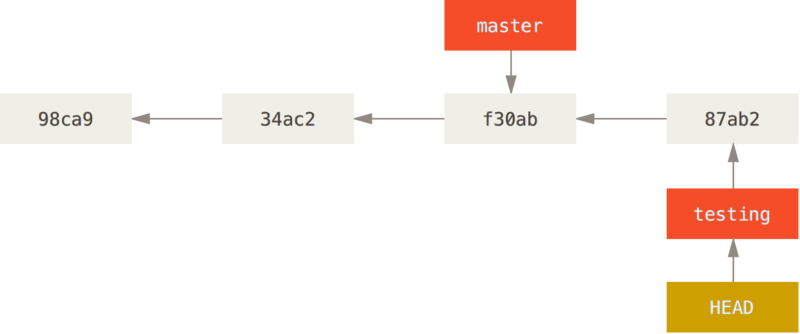
\includegraphics[width=\textwidth]{img/advance-testing.png}
    \end{center}
\end{frame}


\begin{frame}[fragile]
    \frametitle{Branches divergentes}
    \begin{itemize}
        \item Utilité: travailler sur des modifications indépendantes.
    \end{itemize}
\begin{lstlisting}
$ git checkout master
$ [Quelques changements]
$ git commit
\end{lstlisting}
    \begin{center}
        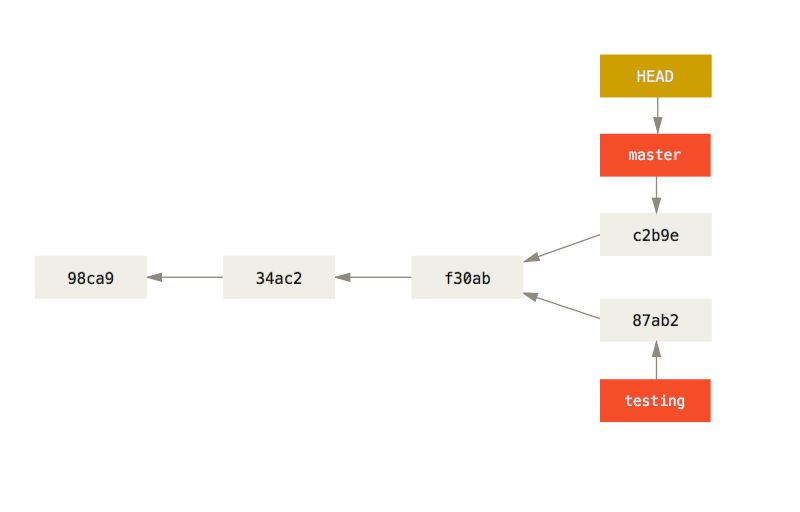
\includegraphics[width=0.8\textwidth]{img/advance-master.png}
    \end{center}
\end{frame}

\begin{frame}[fragile]
\begin{lstlisting}
$ git log --oneline --decorate --graph --all
* c2b9e (HEAD, master) made other changes
| * 87ab2 (testing) made a change
|/
* f30ab add feature #32 - ability to add new formats to the
* 34ac2 fixed bug #1328 - stack overflow under certain conditions
* 98ca9 initial commit of my project
\end{lstlisting}
\end{frame}

\begin{frame}[fragile]
    \frametitle{Commande: git merge: fusionner des modifications}
\begin{lstlisting}
$ git checkout master
Switched to branch 'master'
$ git merge iss53
Merge made by the 'recursive' strategy.
index.html |    1 +
1 file changed, 1 insertion(+)
\end{lstlisting}
\begin{center}
    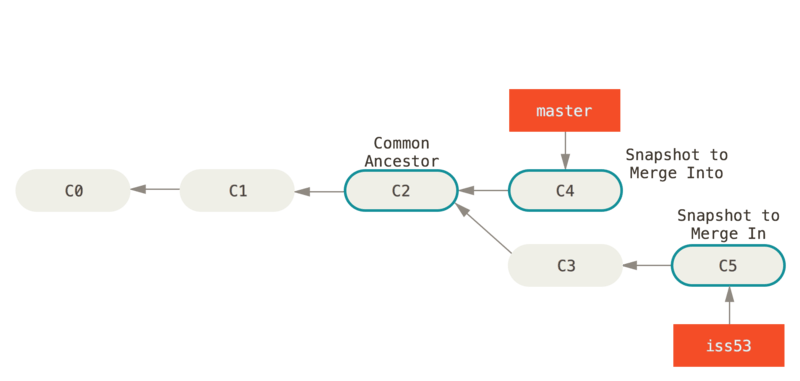
\includegraphics[width=\textwidth,trim=0 0 0 40, clip]{img/basic-merging-1.png}
\end{center}
\end{frame}

\begin{frame}[fragile]
    \frametitle{Commande: git merge (2)}
\begin{lstlisting}
$ git merge iss53
Merge made by the 'recursive' strategy.
index.html |    1 +
1 file changed, 1 insertion(+)
\end{lstlisting}
\begin{center}
    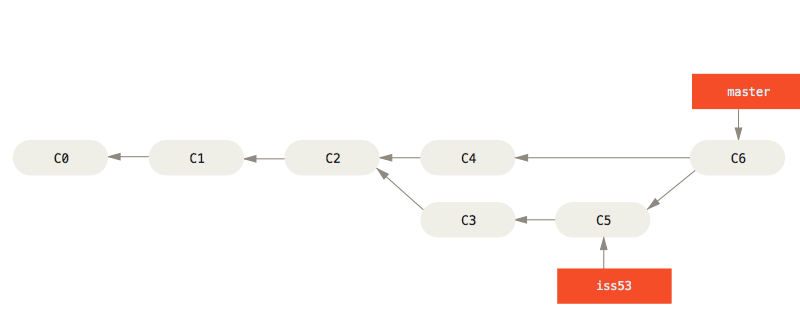
\includegraphics[width=\textwidth,trim=0 0 0 40, clip]{img/basic-merging-2.png}
\end{center}
\end{frame}

\begin{frame}[fragile]
    \frametitle{Conflits}
\begin{lstlisting}
$ git merge iss53
Auto-merging index.html
CONFLICT (content): Merge conflict in index.html
Automatic merge failed; fix conflicts and then commit the result.
$ git status
On branch master
You have unmerged paths.
  (fix conflicts and run "git commit")
Unmerged paths:
  (use "git add <file>..." to mark resolution)
    both modified:      index.html
no changes added to commit (use "git add" and/or "git commit -a")
\end{lstlisting}
\end{frame}

\begin{frame}[fragile]
    \frametitle{Conflits: résolution}
\begin{lstlisting}
<<<<<<< HEAD:index.html
<div id="footer">contact : email.support@github.com</div>
=======
<div id="footer">
 please contact us at support@github.com
>>>>>>> iss53:index.html
\end{lstlisting}
\textbf{Editer le fichier}, ou
(\textbf{Attention}: supprime les modifications de la branche mergée !)
\lstinline{$ git checkout -- [fichier en conflit]}.
Puis
\begin{lstlisting}
$ git add [fichier en conflit]
$ git commit
\end{lstlisting}
\end{frame}

\begin{frame}{Exercice: les branches}

    \begin{itemize}
        \item Les instructions pour les exercices sont à
        \url{https://github.com/louvainlinux/atelier-git/blob/master/instructions.md}.
    \item Essayez de le faire sans la solution.
    \item N'hésitez pas à poser des questions !
    \end{itemize}
\end{frame}

\section{Le travail en groupe}

\begin{frame}{Github, Bitbucket, Gitlab}
\begin{figure}
    \centering
    
\includegraphics[width=0.7\textwidth]{img/github-bitbucket.png} \\
    
\includegraphics[width=0.6\textwidth]{img/gitlab.png}
\end{figure}
\end{frame}

\begin{frame}{Distribué... comment se synchroniser ?}
    \begin{center}
        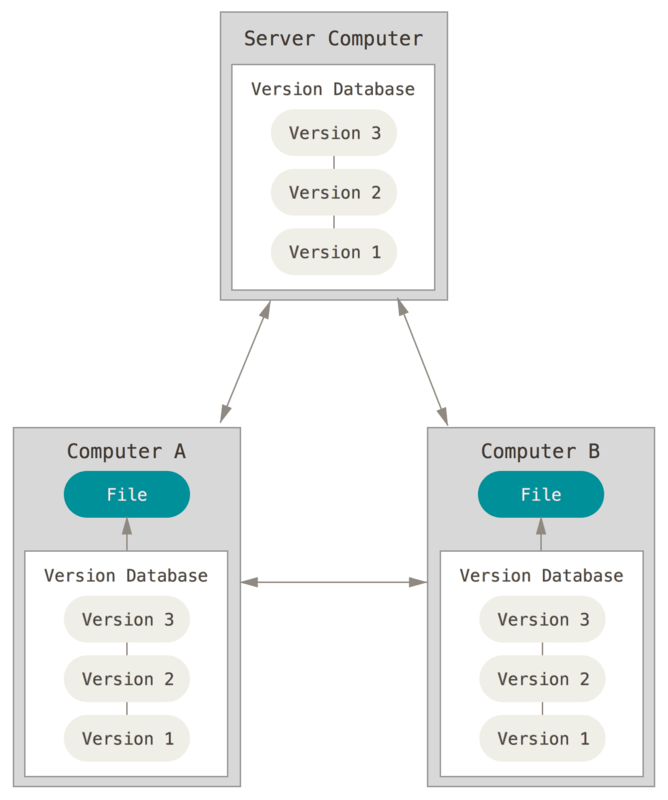
\includegraphics[width=0.6\textwidth]{img/distributed.png}
    \end{center}
\end{frame}

\begin{frame}{Mise en place}
    \begin{center}
        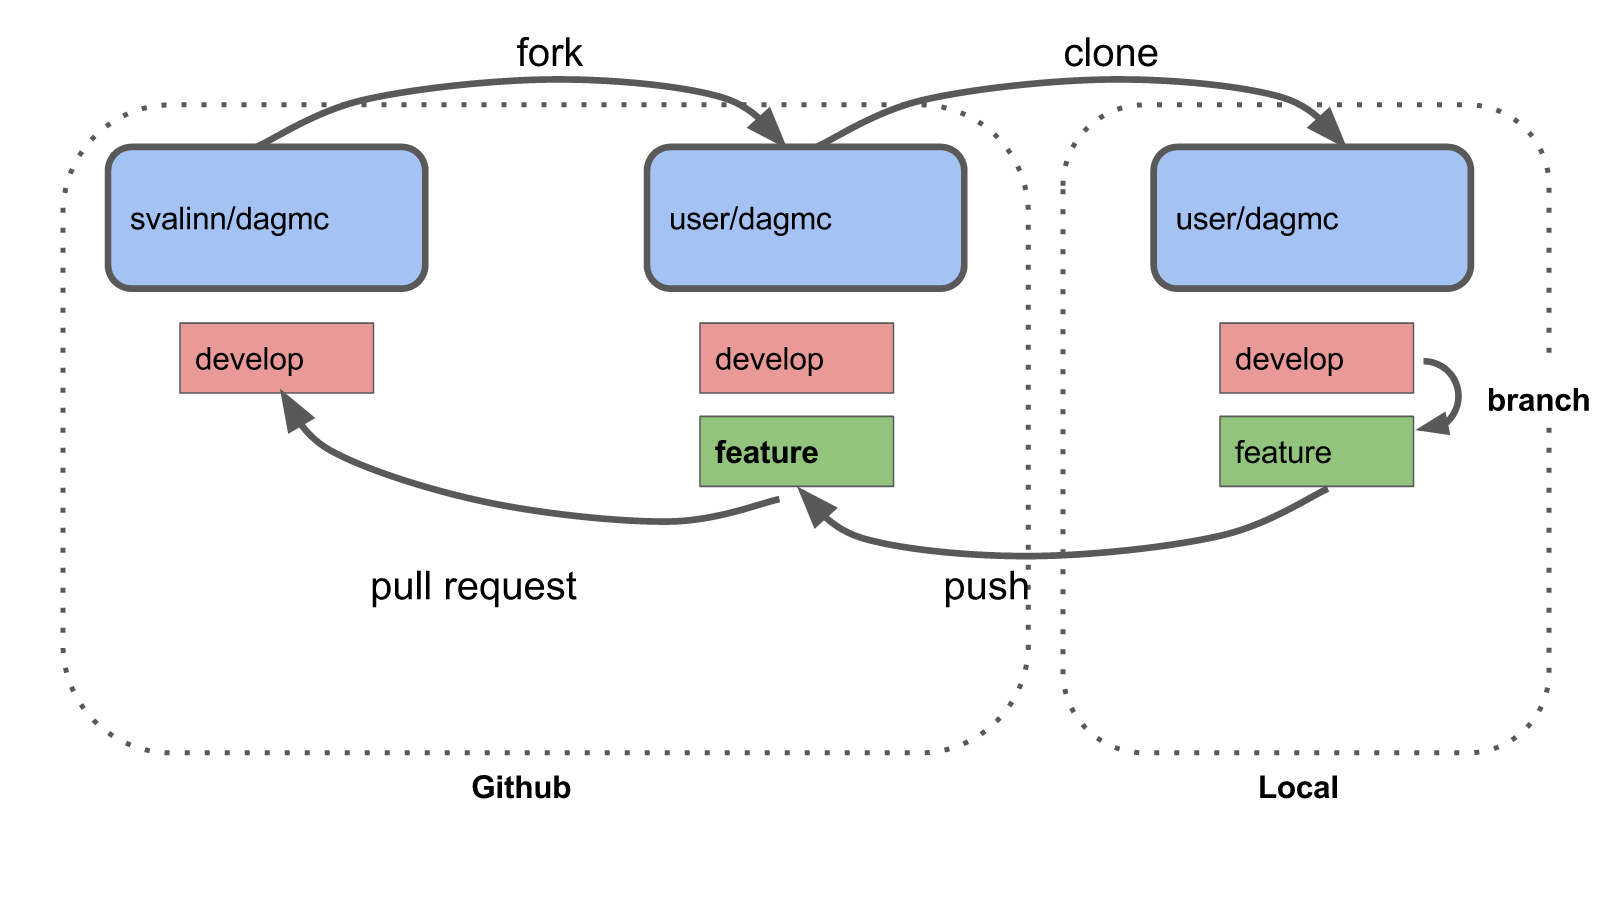
\includegraphics[width=\textwidth]{img/github-setup.png}
    \end{center}
\end{frame}

\begin{frame}{Méthode de travail}
    \begin{center}
        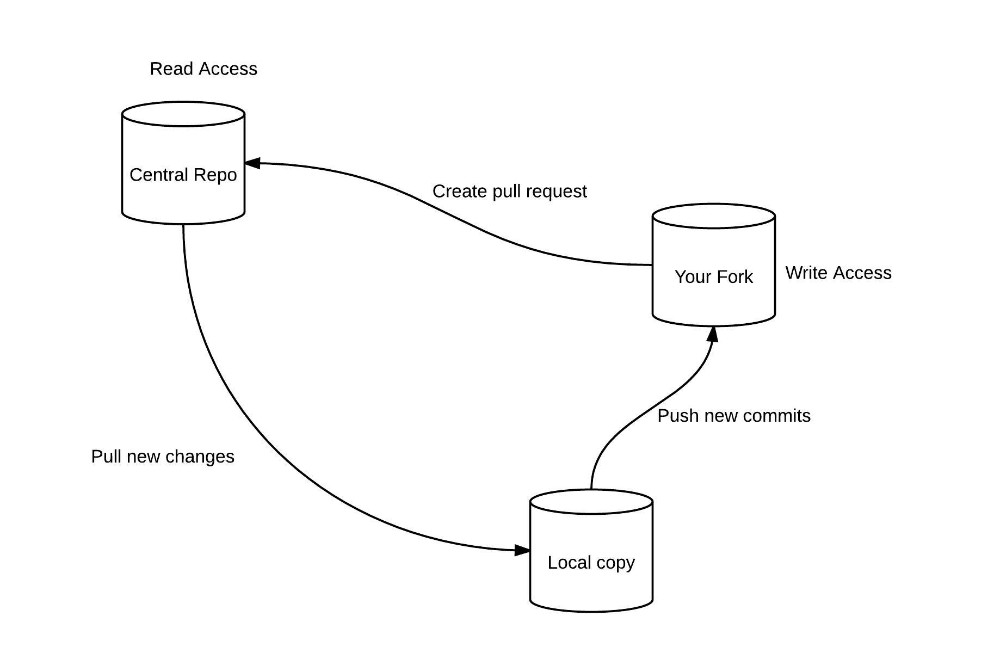
\includegraphics[width=\textwidth]{img/github-workflow.jpg}
    \end{center}
\end{frame}

\begin{frame}[fragile]
\frametitle{git clone}

\begin{itemize}
\item Cloner un répertoire \texttt{git} depuis un serveur principal
\item Exemple
\begin{lstlisting}
git clone <url>
\end{lstlisting}
\end{itemize}
\end{frame}

\begin{frame}[fragile]
\frametitle{git remote}

\begin{itemize}
\item Ajouter un serveur distant à votre répertoire \texttt{git}
\item Exemple
\begin{lstlisting}
git remote add origin <url>
\end{lstlisting}
\end{itemize}
\end{frame}


\begin{frame}[fragile]
\frametitle{git pull}

\begin{itemize}
\item Récupérer les dernières modifications depuis le serveur principal
\item Exemple
\begin{lstlisting}
git pull origin
\end{lstlisting}
\end{itemize}
\end{frame}

\begin{frame}[fragile]
\frametitle{git push}

\begin{itemize}
\item Envoyer les dernières modifications locales sur le serveur principal
\item Exemple
\begin{lstlisting}
git push origin master
\end{lstlisting}
\end{itemize}
\end{frame}

\begin{frame}[fragile]
\frametitle{Exemple de collaboration avec GitHub}
  \begin{center}
      
\includegraphics[width=\textwidth]{img/github_home}
  \end{center}
\end{frame}

\begin{frame}[fragile]
\frametitle{Exemple avec GitHub}
  \begin{center}
      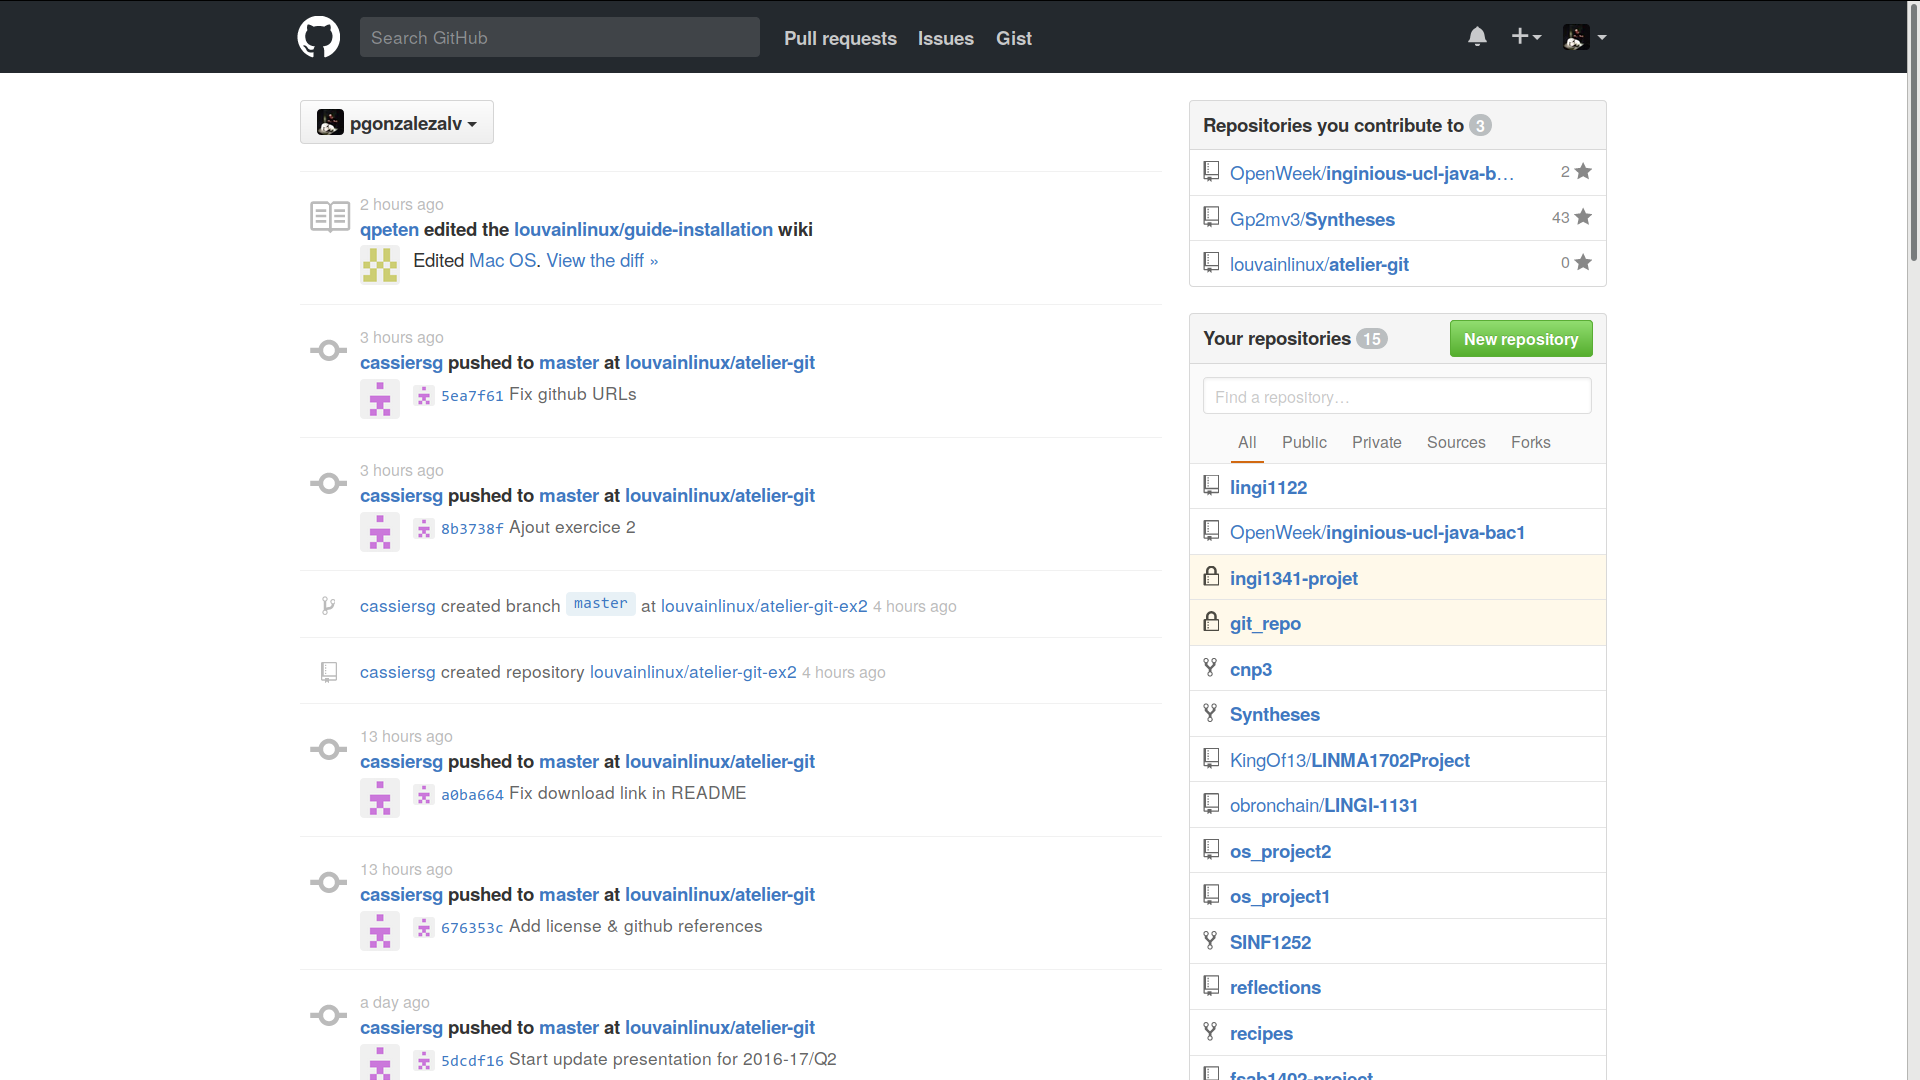
\includegraphics[width=\textwidth]{img/github_account_home}
  \end{center}
\end{frame}

\begin{frame}[fragile]
\frametitle{Exemple avec GitHub}
  \begin{center}
      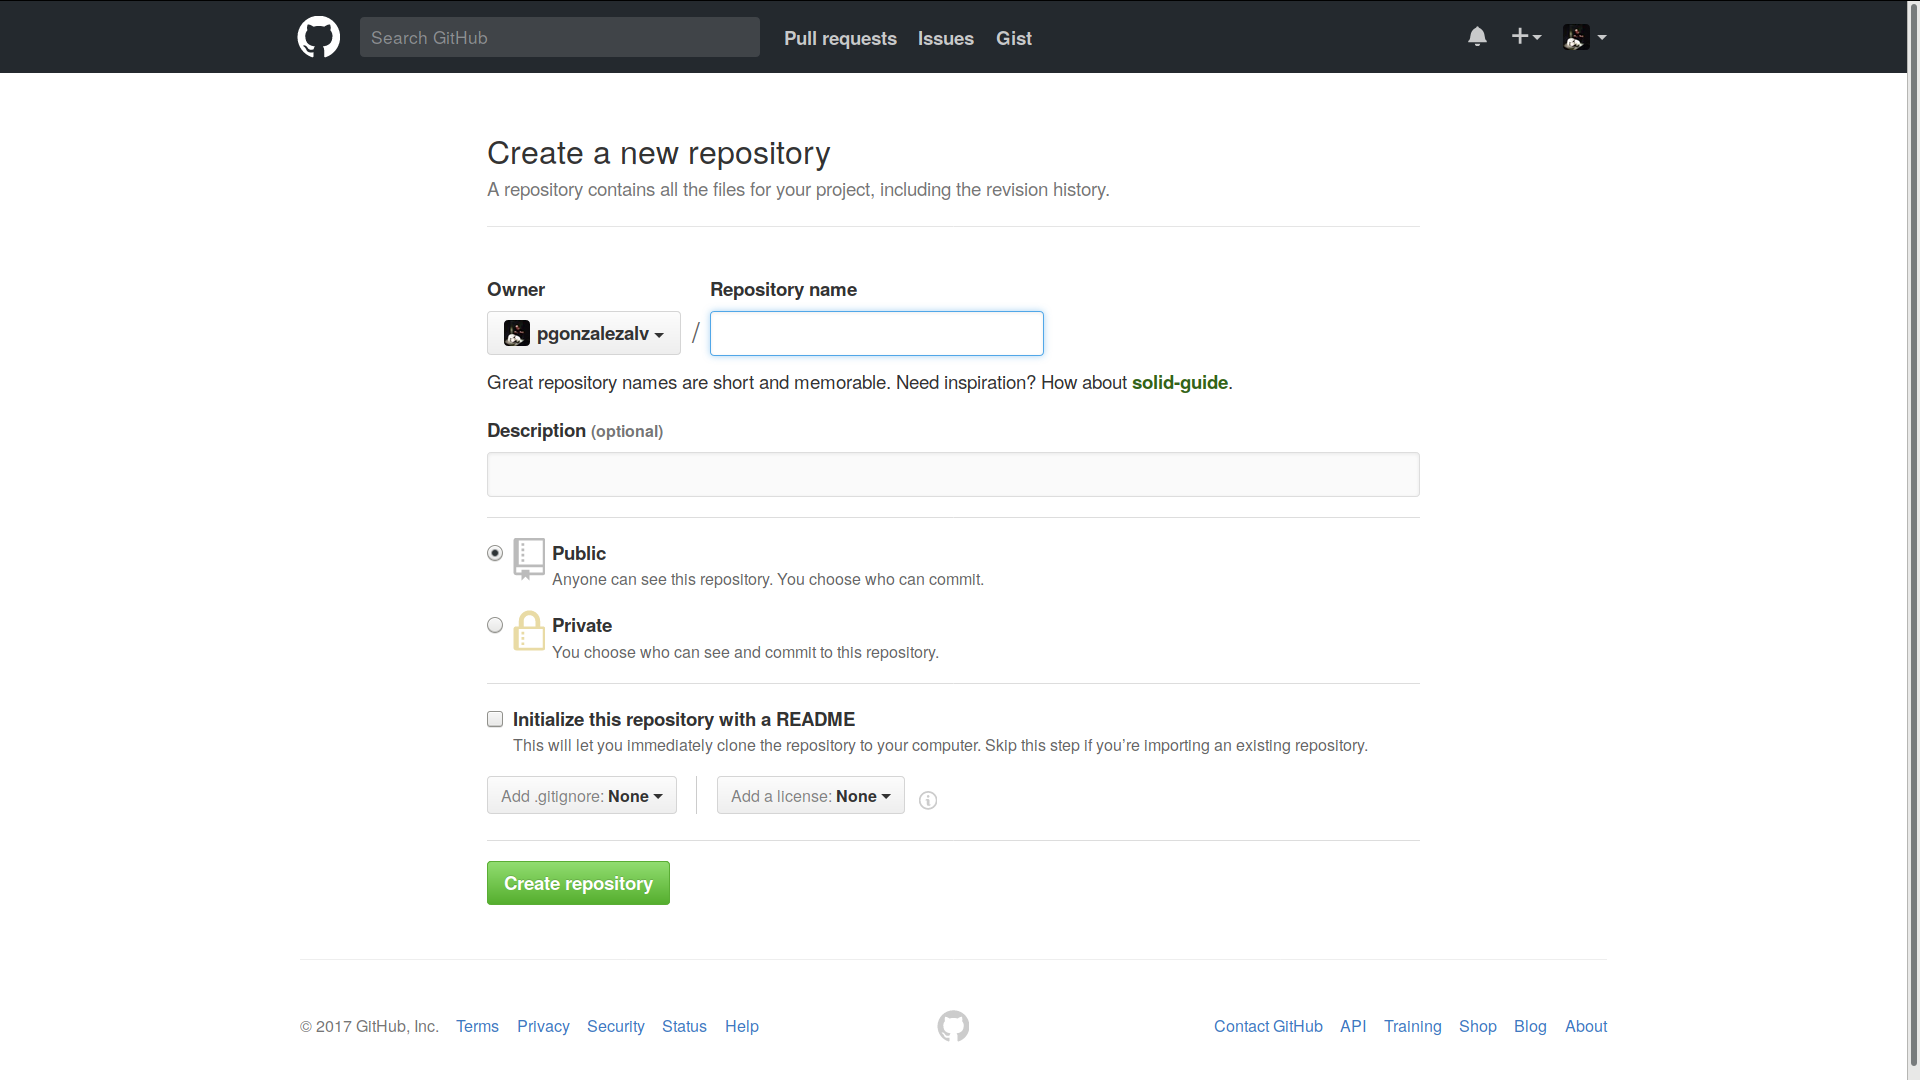
\includegraphics[width=\textwidth]{img/github_new_project}
  \end{center}
\end{frame}

\begin{frame}[fragile]
\frametitle{Exemple avec GitHub}
  \begin{center}
      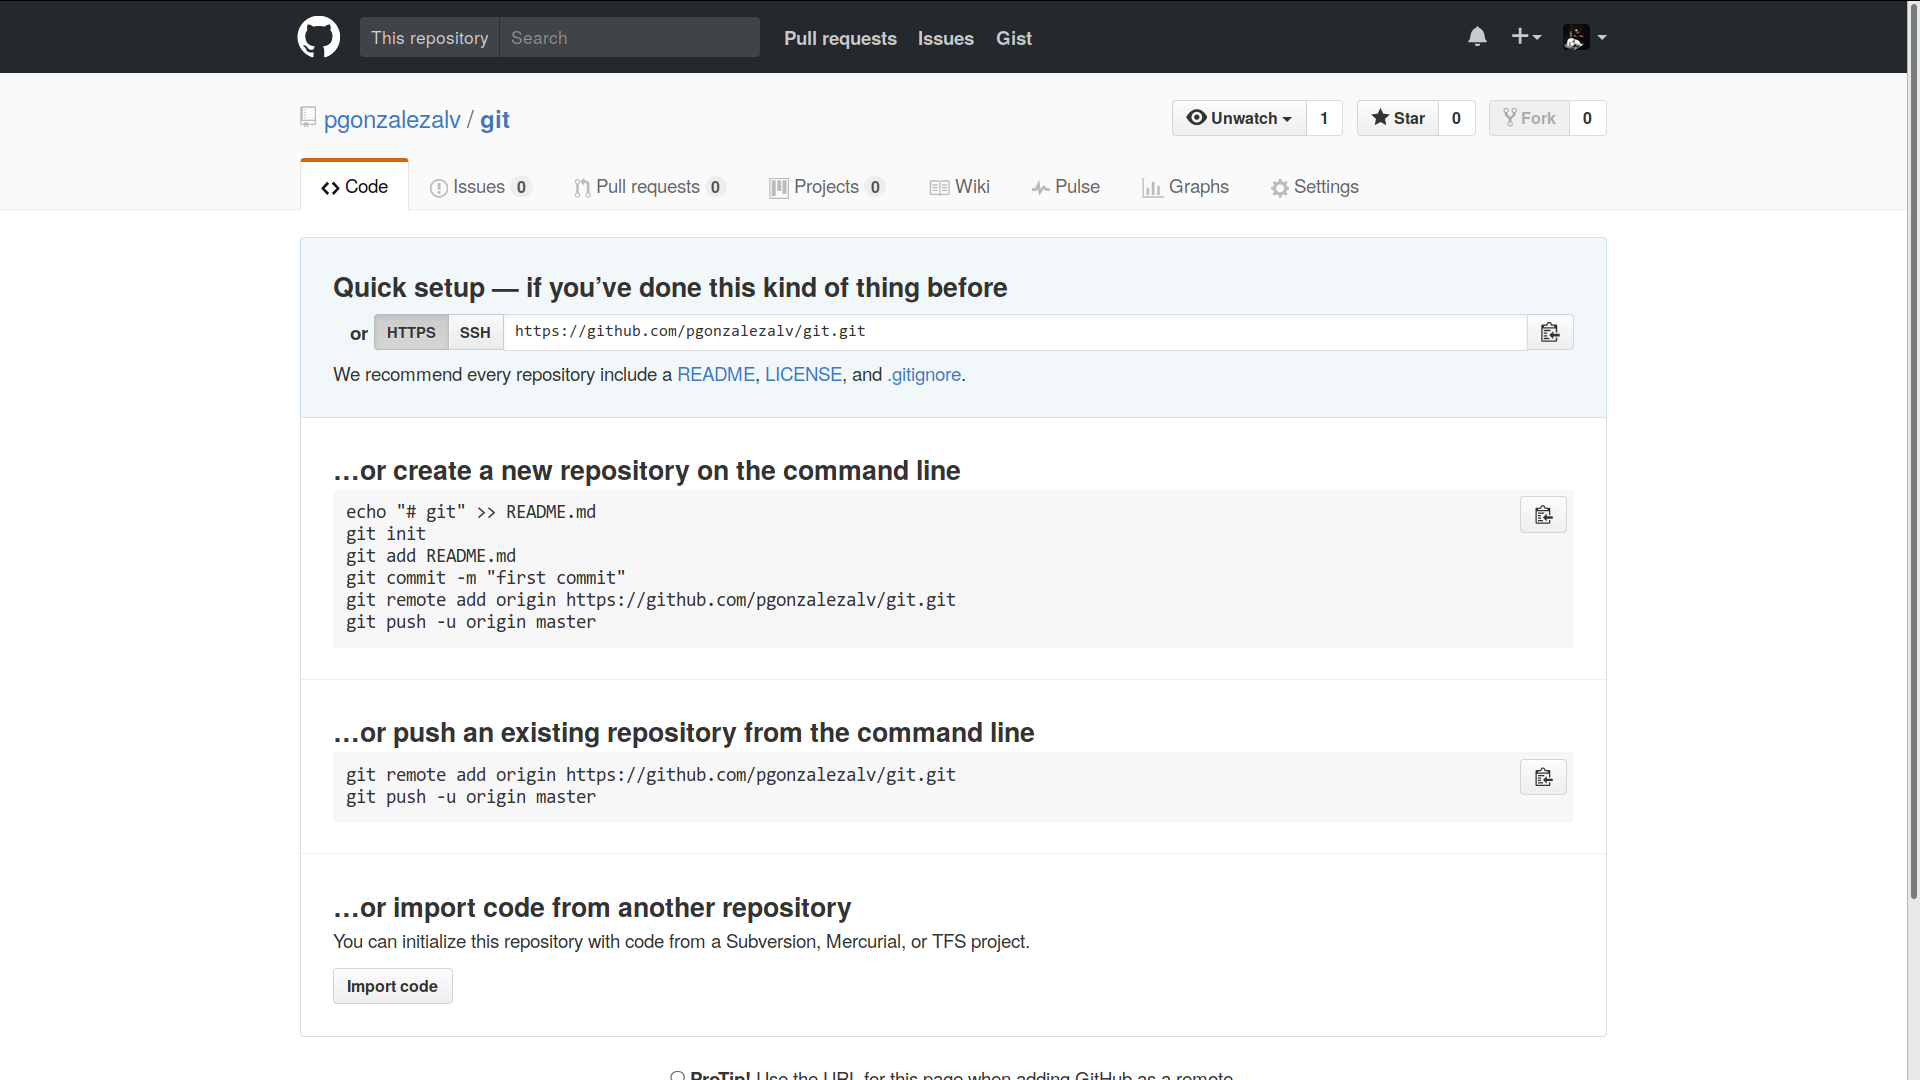
\includegraphics[width=\textwidth]{img/github_new_project_setup}
  \end{center}
\end{frame}

\begin{frame}[fragile]
\frametitle{Exemple avec GitHub}
  \begin{center}
      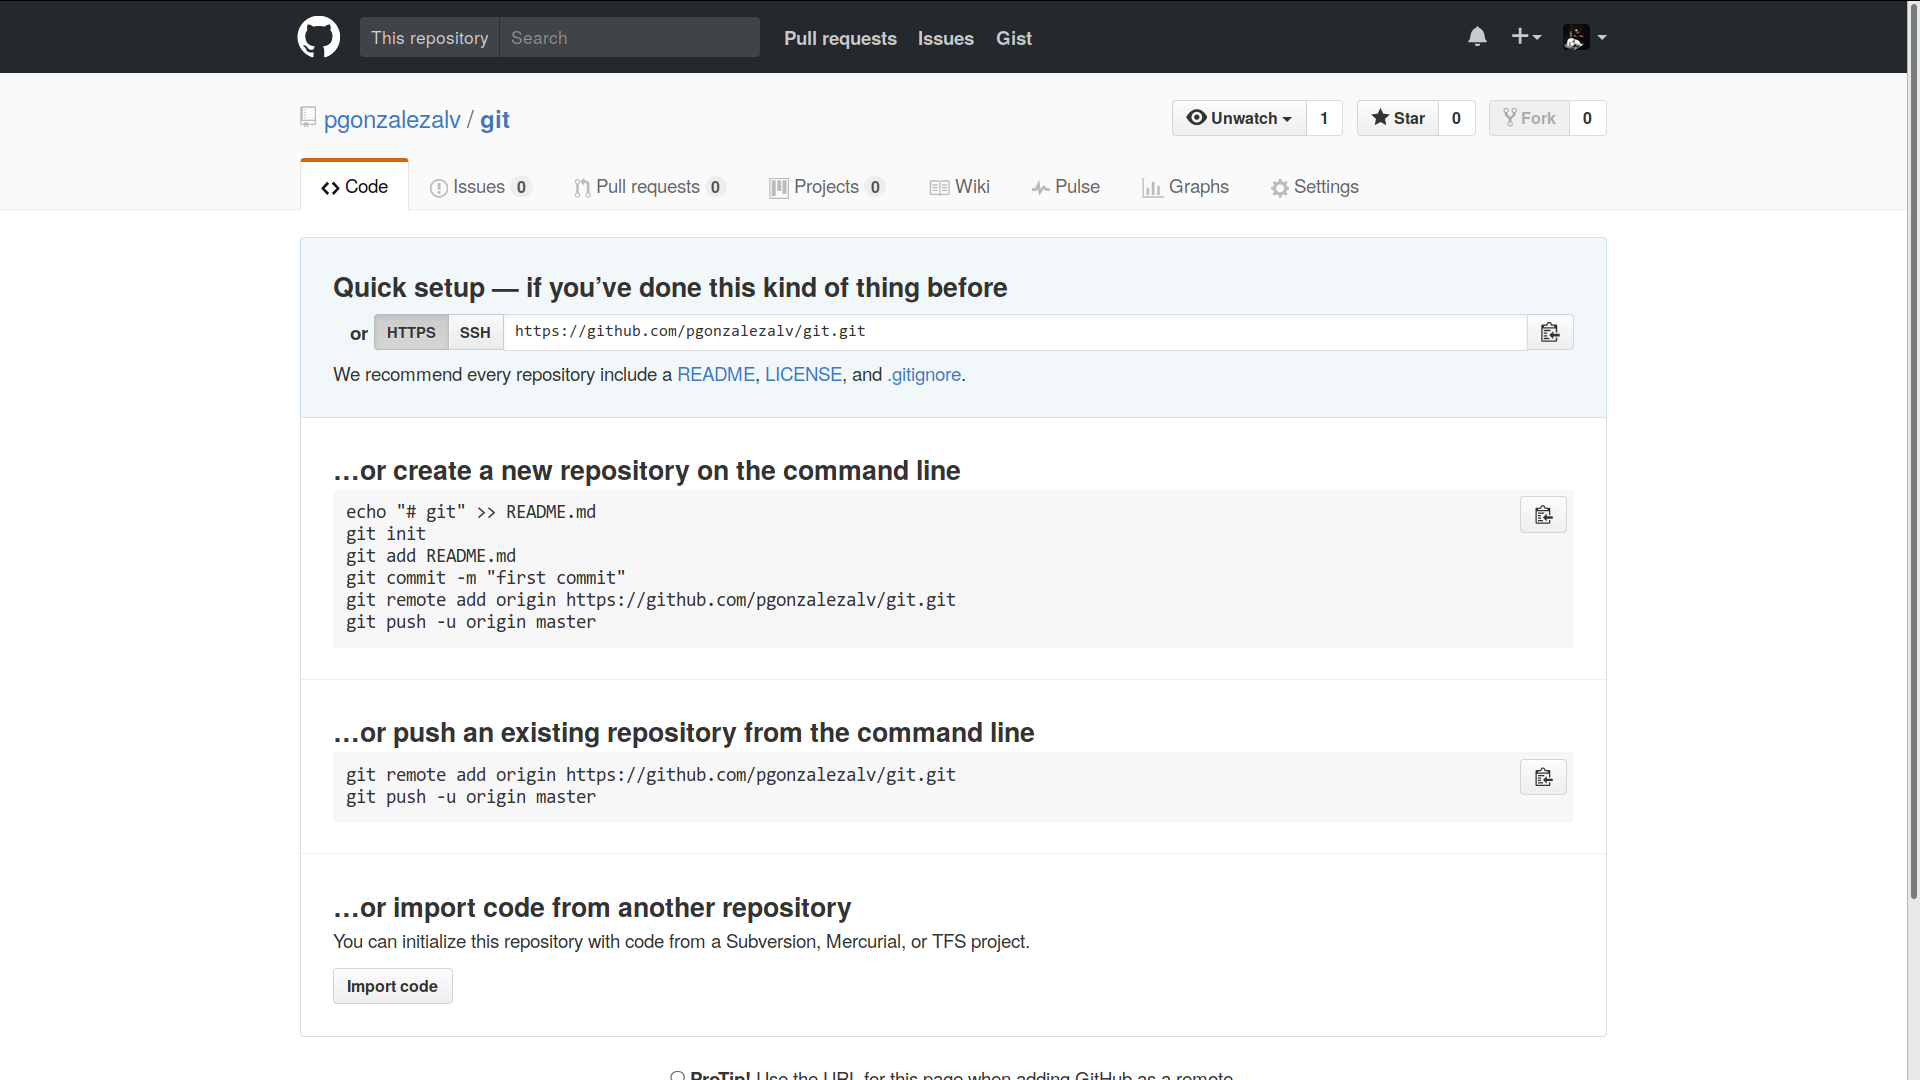
\includegraphics[width=\textwidth]{img/github_new_project_setup}
  \end{center}
\end{frame}

\begin{frame}[fragile]
\frametitle{Exemple avec GitHub}
  \begin{center}
      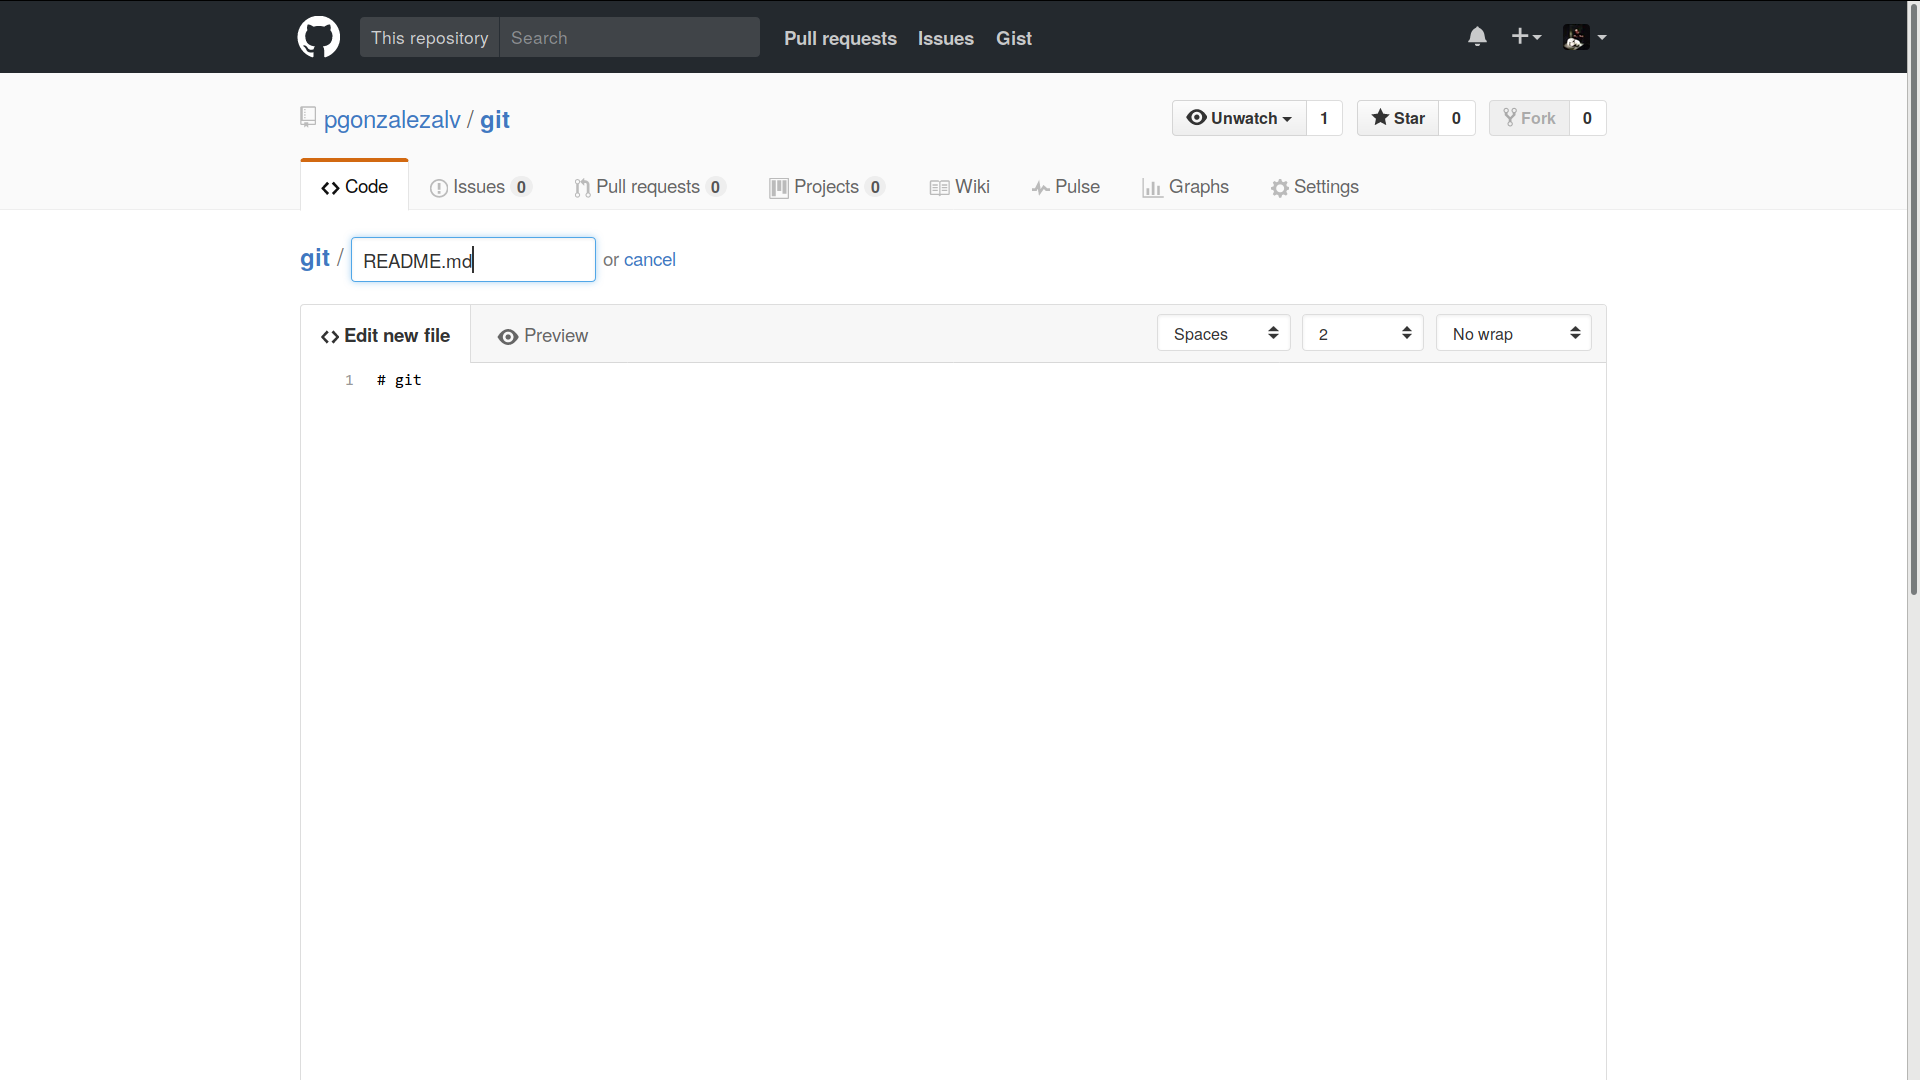
\includegraphics[width=\textwidth]{img/github_new_project_readme}
  \end{center}
\end{frame}

\begin{frame}[fragile]
\frametitle{Exemple avec GitHub}
  \begin{center}
      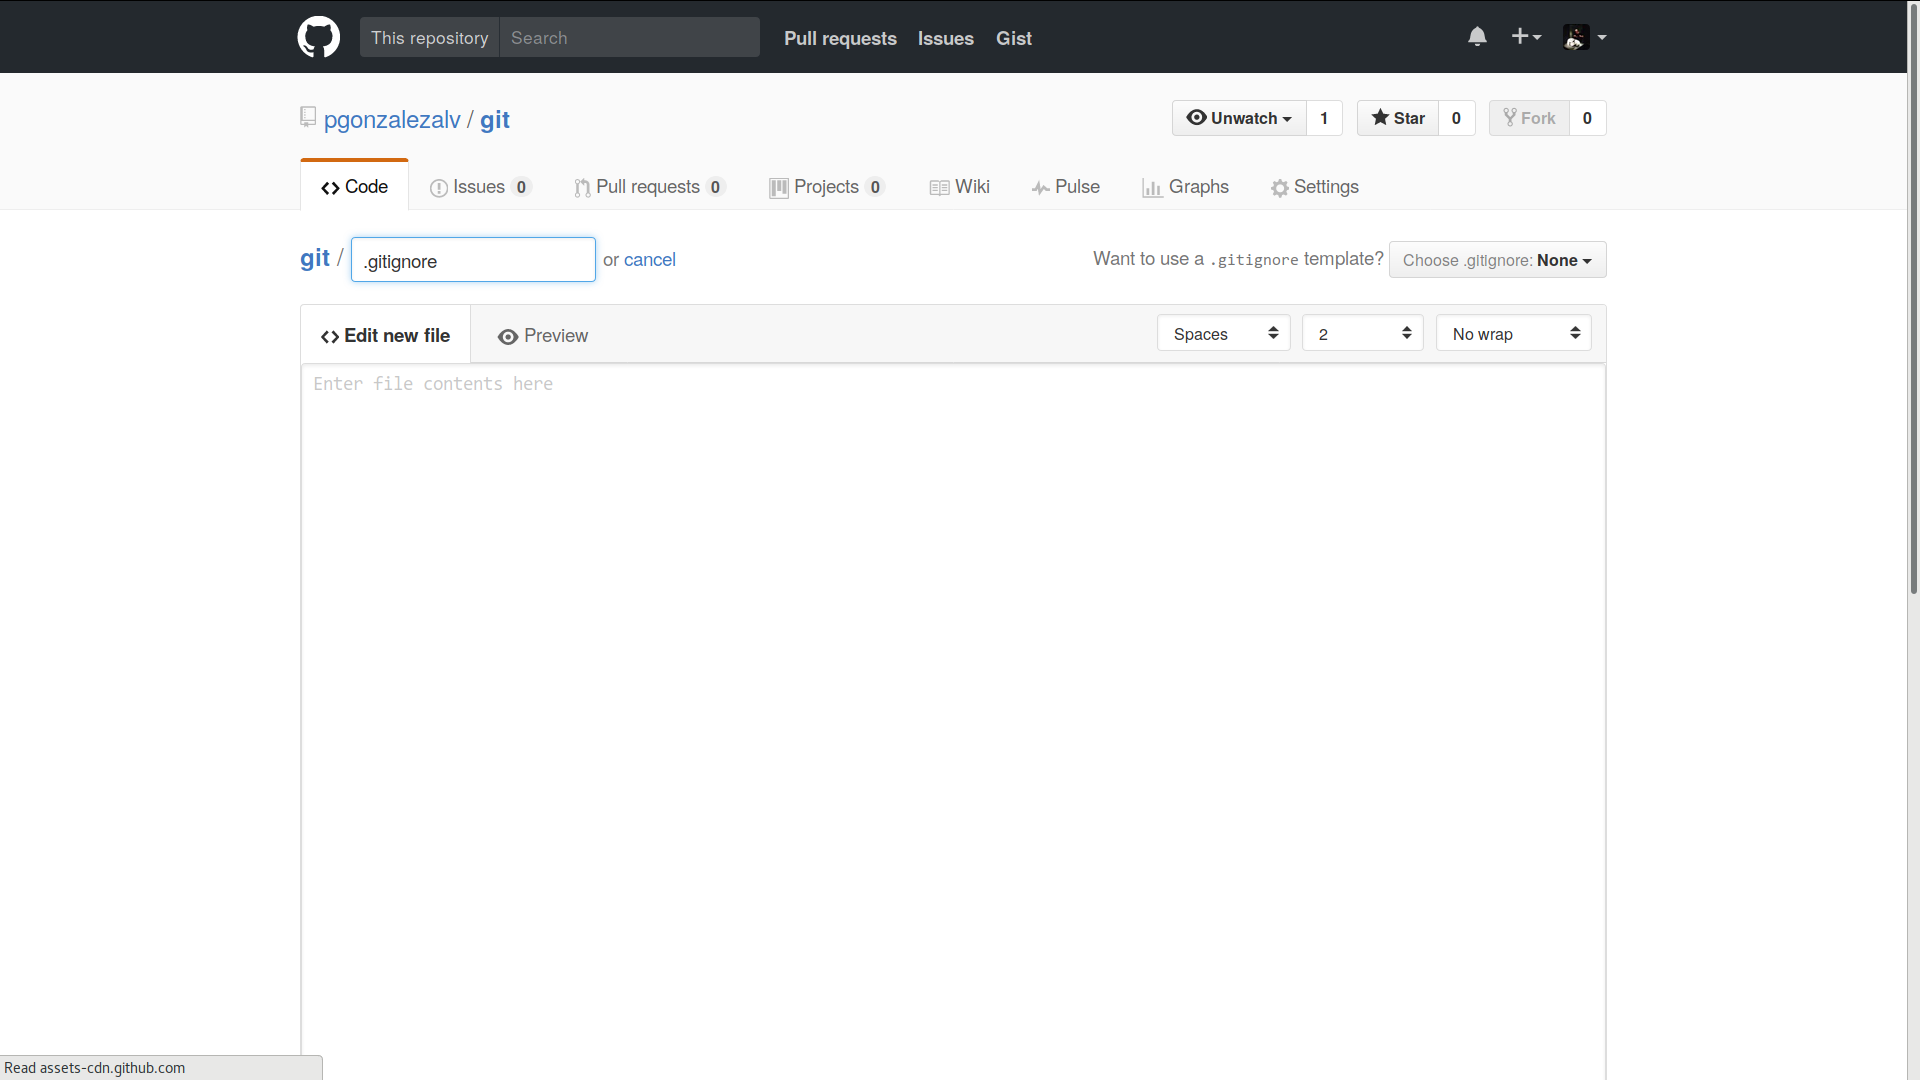
\includegraphics[width=\textwidth]{img/github_new_project_gitignore}
  \end{center}
\end{frame}

\begin{frame}[fragile]
\frametitle{Exemple avec GitHub}
  \begin{center}
      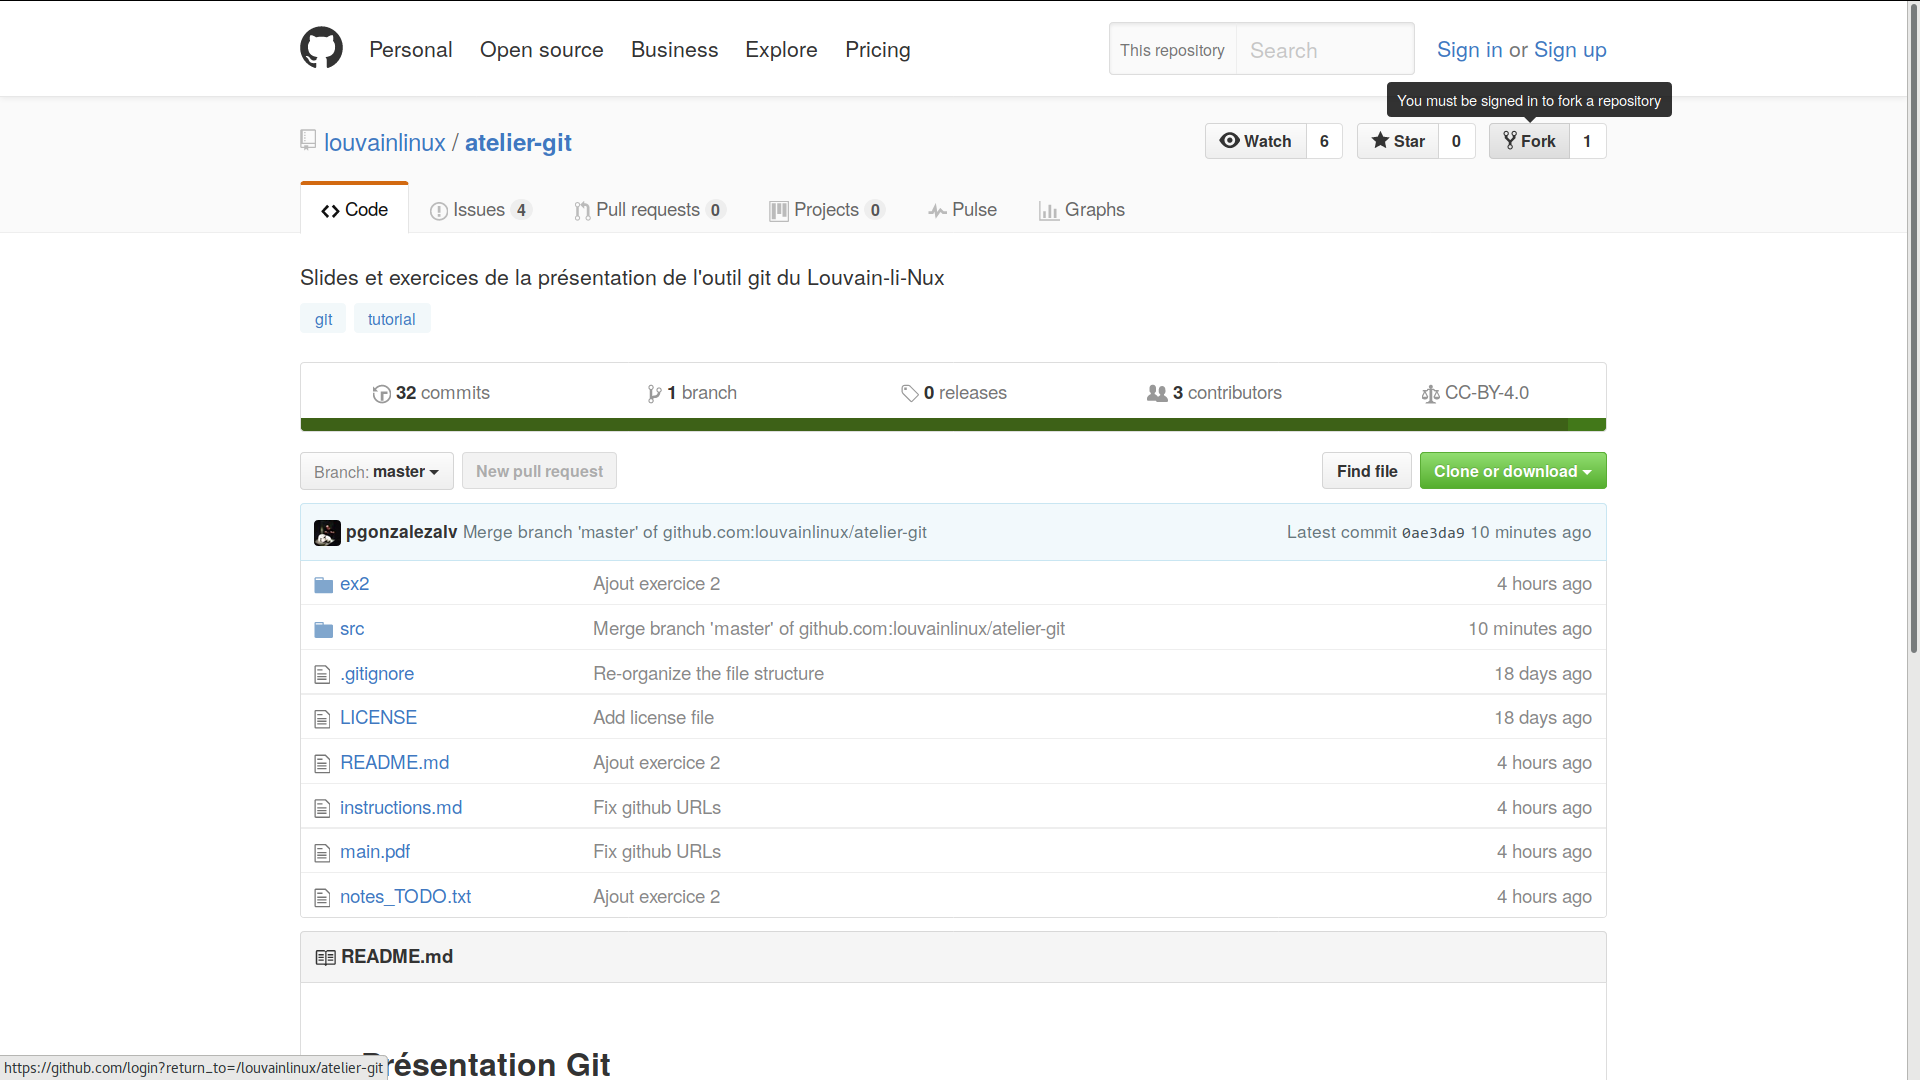
\includegraphics[width=\textwidth]{img/github_new_project_fork}
  \end{center}
\end{frame}

\begin{frame}[fragile]
\frametitle{Exemple avec GitHub}
  \begin{center}
      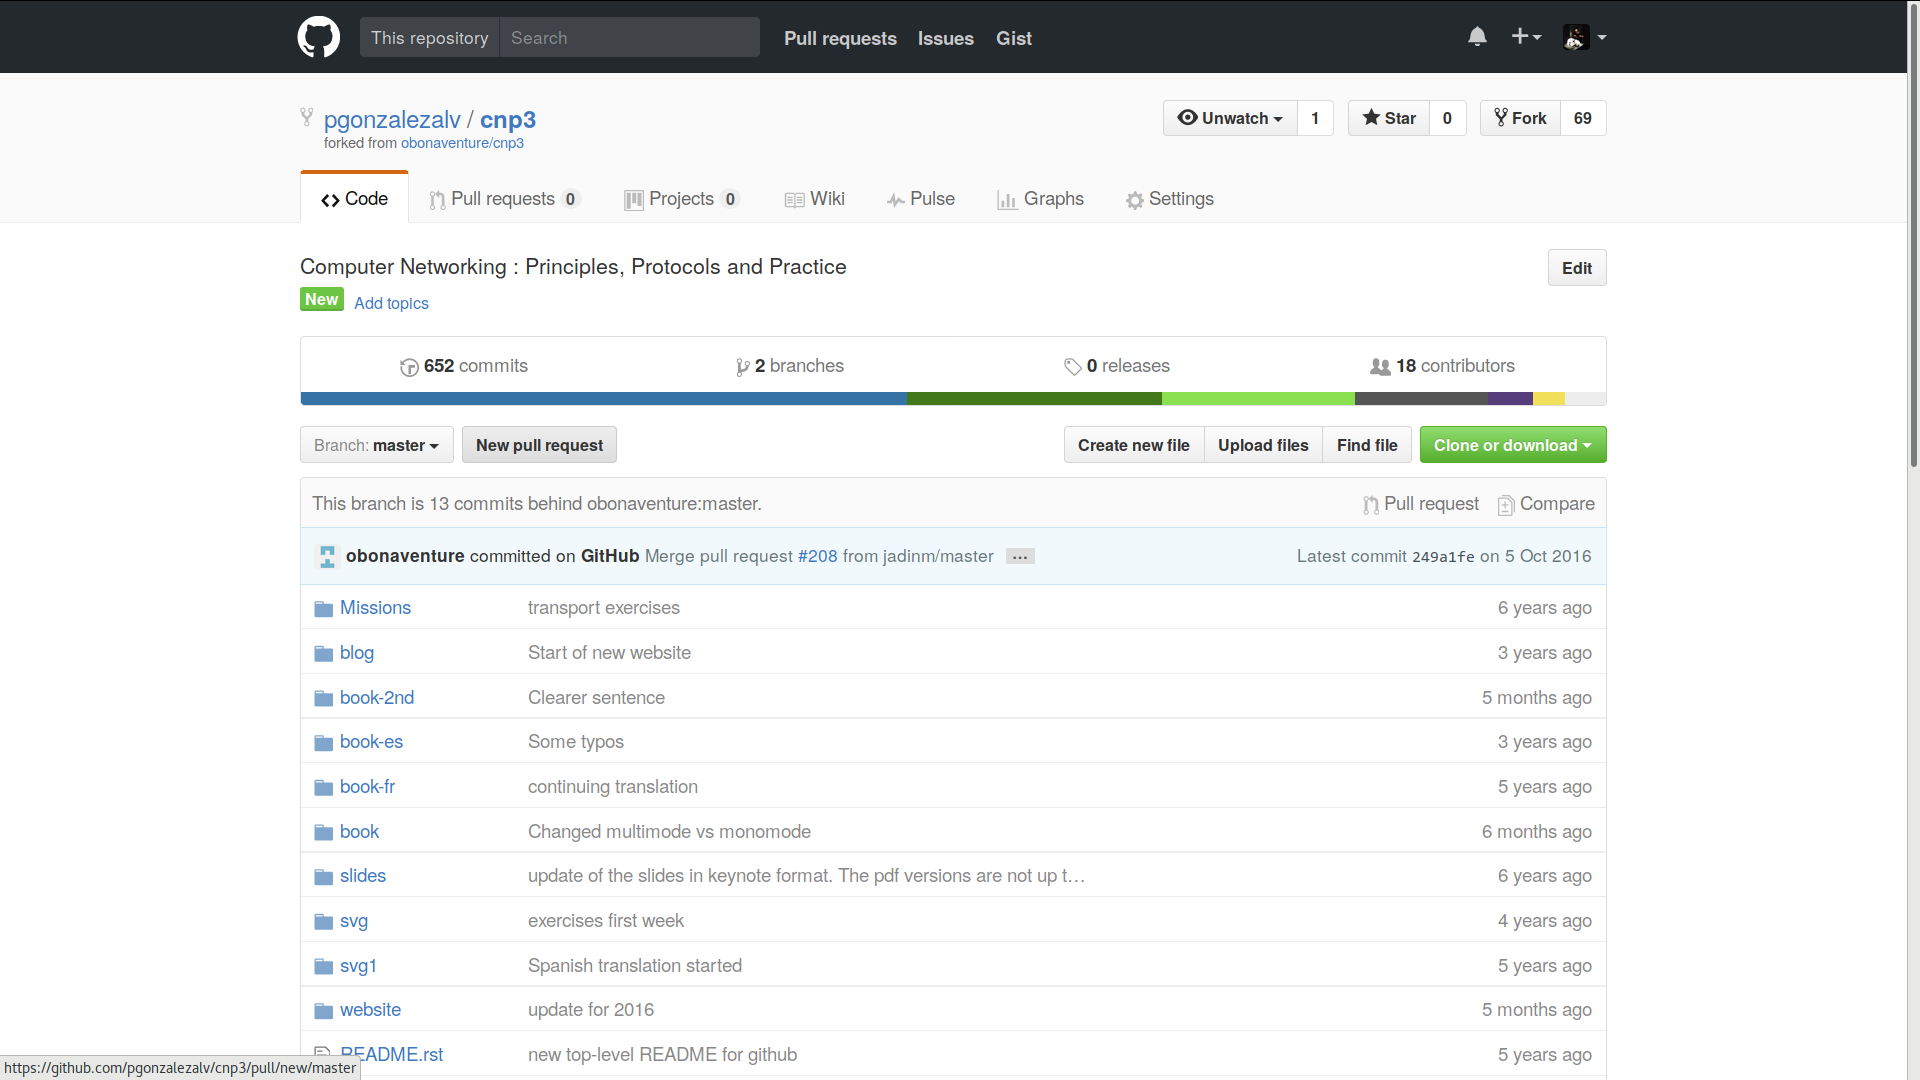
\includegraphics[width=\textwidth]{img/github_pull_request}
  \end{center}
\end{frame}

\begin{frame}[fragile]
\frametitle{Exemple avec GitHub}
  \begin{center}
      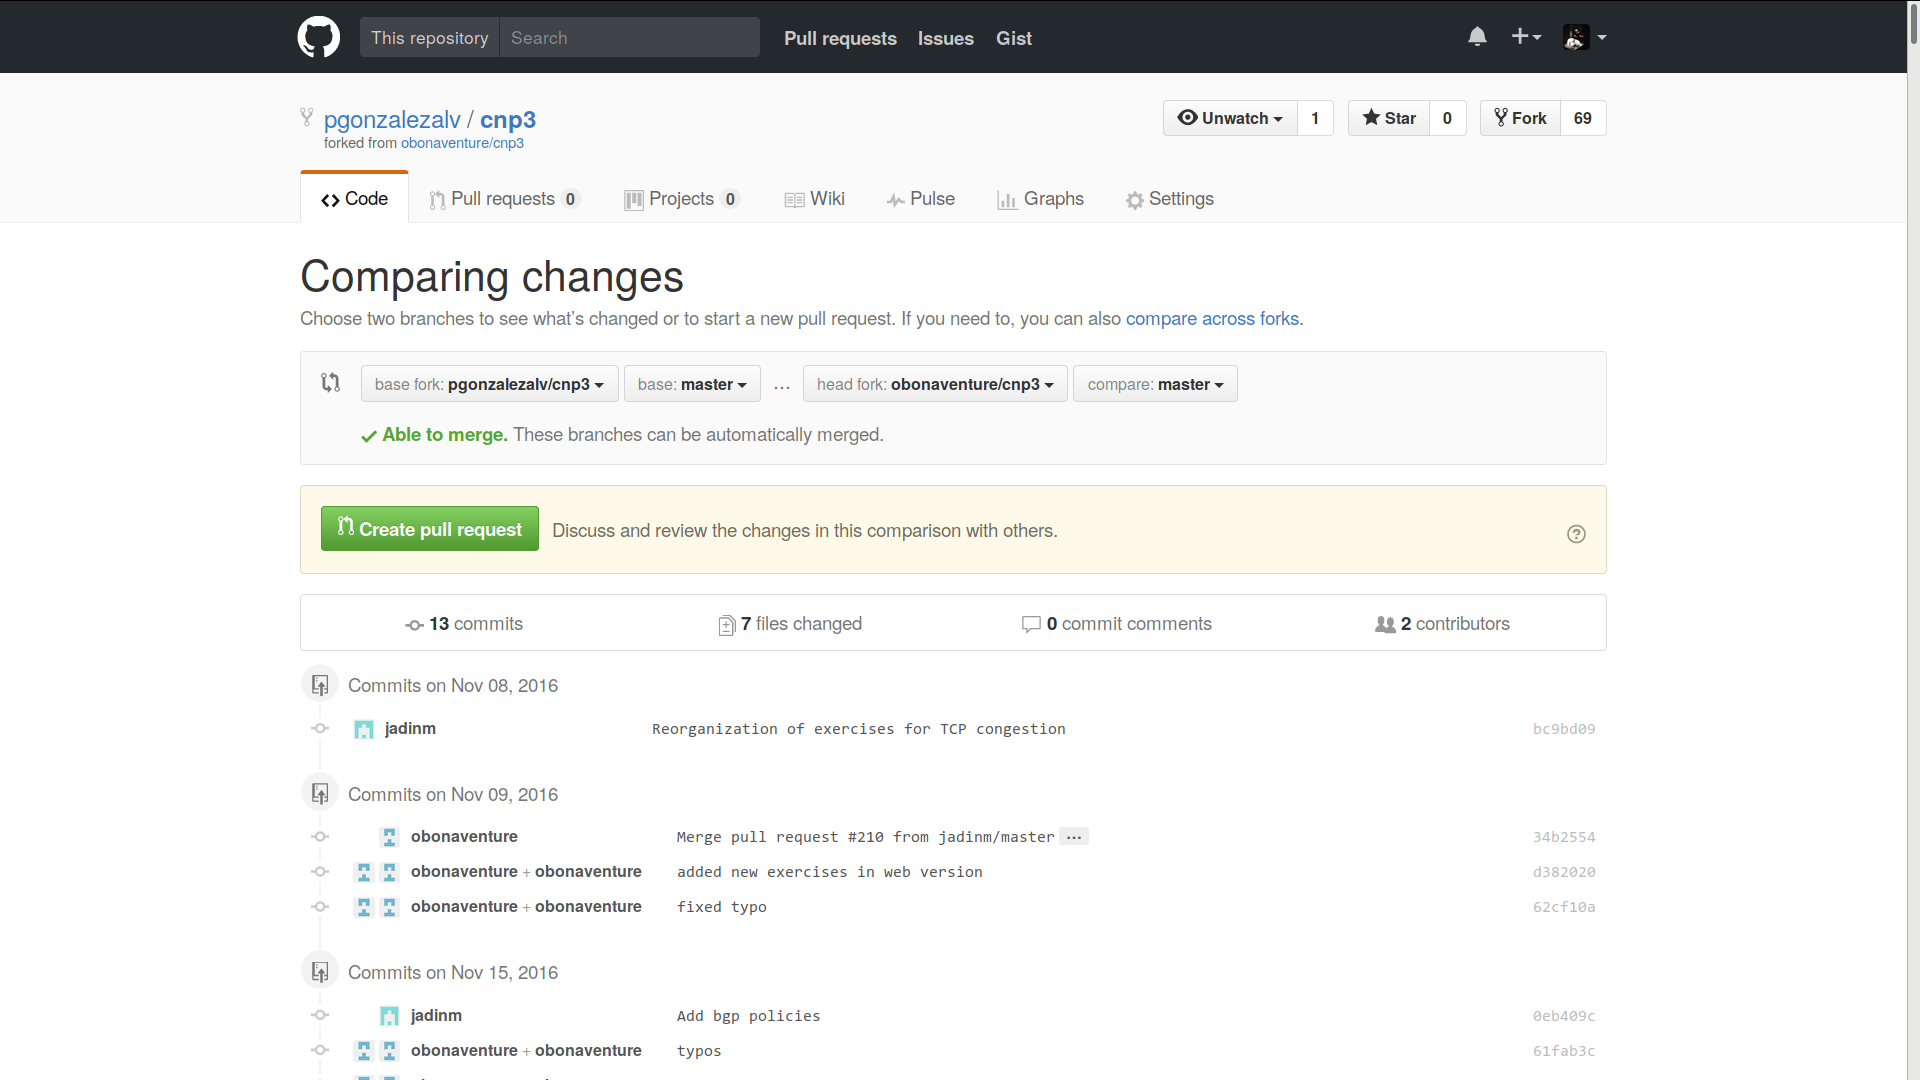
\includegraphics[width=\textwidth]{img/github_pull_request_cmp}
  \end{center}
\end{frame}

\begin{frame}[fragile]
\frametitle{Exemple avec GitHub -- Les commandes utiles}
\begin{lstlisting}
$ git clone https://github.com/username/repo_name.git # pour cloner un repo git depuis GitHub
$ git add remote origin https://github.com/username/repo_name.git # pour ajouter un repo GitHub a un repo git existant
$ git pull origin master # pour recuperer les modifications sur le repo GitHub
$ git push origin master # pour envoyer des modifications sur le repo GitHub
\end{lstlisting}
\end{frame}

\begin{frame}{Pour aller plus loin ...}

Références
\begin{itemize}
    \item \textbf{La référence: Git book}: \url{https://git-scm.com/book}
    \item Github help: \url{https://help.github.com/}
\end{itemize}

GUI
    \begin{itemize}
        \item \url{https://git-scm.com/docs/gitk} (Installé par défaut sous Windows)
      \item \url{https://www.gitkraken.com/}
      \item \url{https://desktop.github.com/}
      \item D'autres: \url{https://git-scm.com/downloads/guis}
    \end{itemize}
Github Student Pack
\begin{itemize}
    \item \url{https://education.github.com/pack}
\end{itemize}
\end{frame}

\plain{Questions?}
\end{document}
